\documentclass[prd,showpacs,preprintnumbers,amsmath,amssymb,twocolumn,
superscriptaddress,notitlepage]{revtex4-2}

%\pdfoutput=1
\usepackage{cases}
\usepackage{amsmath}
\usepackage{amssymb}
\usepackage{amsfonts}
\usepackage{amssymb}
\usepackage{dcolumn}
\usepackage{bm}
\usepackage{epsfig}
\usepackage{bbm}
\usepackage{graphicx}
\usepackage{xcolor}
\usepackage{array}
\usepackage{mathrsfs}
\usepackage{verbatim}
\usepackage{epstopdf}
\usepackage{color}
\usepackage{orcidlink}
\usepackage{comment}


\newcommand{\bra}[1]{\langle #1\vert}
\newcommand{\ket}[1]{\vert #1\rangle}
\newcommand{\be}{\begin{equation}}
\newcommand{\ee}{\end{equation}}
\newcommand{\ba}{\begin{eqnarray}}
\newcommand{\ea}{\end{eqnarray}}
\newcommand{\nn}{\nonumber \\}
\newcommand{\lag}{\langle}
\newcommand{\rag}{\rangle}
\newcommand{\cN}{{\cal N}}
\newcommand{\cA}{{\cal A}}
\newcommand{\gsim}{\mathrel{\hbox{\rlap{\lower.55ex \hbox {$\sim$}}
			\kern-.3em \raise.4ex \hbox{$>$}}}}
\newcommand{\lsim}{\mathrel{\hbox{\rlap{\lower.55ex \hbox {$\sim$}}
			\kern-.3em \raise.4ex \hbox{$<$}}}}

\usepackage{ulem,fancyvrb}
\usepackage{hyperref}
\usepackage{xcolor} 
\newcommand{\zb}[1]{{\color{blue} {#1}}}
\newcommand{\zr}[1]{{\color{red} {#1}}}
\newcommand{\zd}[1]{{\color{red}{\sout{#1}}}}
\newcommand{\zc}[1]{{\color{blue} {#1}}}
\newcommand{\zx}[2]{{\color{red}{\sout{#1}}}~{\color{blue}{#2}}}
\newcommand{\WXP}[1]{\textcolor{purple} {WXP: #1}}
\newcommand{\jl}[1]{\textcolor{orange} {jl: #1}}


\hypersetup{colorlinks=true,
	breaklinks=true,
	pdfstartview=Fit,
	linkcolor=blue,
	citecolor=blue,
	urlcolor=blue,
	pdftitle={3body-for-HDM},
	pdfauthor={Jia Liu}}

\begin{document}
\title{3body-for-HDM} % Provisional working title; confirm the formal title.
\author{Jia Liu}
% No affiliation or contact information is present in the supplied source.
% Add the verified institutional affiliation and email only after confirmation.

\begin{abstract}
% TODO: Add a source-supported summary only after the signal calculation,
% statistical interpretation, and cosmological analysis have been verified.
% Suggested structure: motivation; process; calculation method; key results;
% scope and limitations.
\end{abstract}





\maketitle


\section{Introduction}
% TODO: Establish the LZ experimental context using the exact analysis and
% candidate/event definition; motivate the three-body dark-matter process;
% summarize the research question and state the scope of this work.
% Do not state that the model explains the LZ event until the likelihood and
% competing constraints have been independently validated.

\section{Model}

\subsection{Vector--vector}


We consider a dark sector consisting of two heavy fermions,
$\chi_1$ and $\chi_2$, a massive $U(1)_X$ gauge boson $V_\mu$,
and a light scalar $s$. The relevant interaction Lagrangian is
given by
\begin{equation}
	\begin{aligned}
		\mathcal{L}_{\rm int}
		={}&
		g_1 V^\mu \bar{\chi}_2 \gamma_\mu \chi_1
		+ g_2 s \bar{\chi}_2 \chi_1
		+ \mathrm{h.c.}
		\\
		&+g_{Vq} V^\mu \sum_q \bar q \gamma_\mu q,
	\end{aligned}
	\label{eq:Lint_VV}
\end{equation}
where the sum runs over all quark flavors. Here, $g_1$, $g_2$,
and $g_{Vq}$ denote the corresponding coupling constants. We assume
that the vector mediator couples universally to all quark flavors,
with a flavor-independent coupling $g_{Vq}$. The scalar $s$ is
assumed to have a sub-MeV mass. We assume the mass of $\chi_2$ is slightly heavier than $\chi_1$ and define
\begin{equation}
\Delta m = m_{\chi_2} - m_{\chi_1}.
\end{equation}
The coupling between $V$ and nucleon is then given by
\begin{equation}
g_{VN} = 3 g_{Vq}
\end{equation}

\subsection{Scalar--pseudoscalar}

\begin{equation}
	\begin{aligned}
		\mathcal{L}_{\rm int}
		={}&
		g_1 \phi \bar{\chi}_2 \chi_1
		+ g_2 s \bar{\chi}_2 \chi_1
		+ \mathrm{h.c.}
		\\
		&+ i g_{\phi N} \phi \sum_{N = p,n } \bar{N} \gamma^5 N,
	\end{aligned}
	\label{eq:Lint_SPS}
\end{equation}


\begin{figure*}[t]
    \centering
    \begin{minipage}[t]{0.48\textwidth}
        \centering
        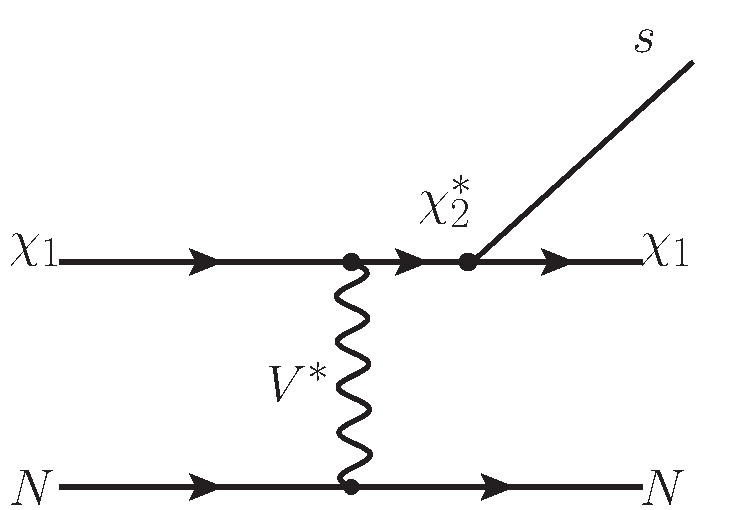
\includegraphics[width=\linewidth]{figures/LZ_3body_DM_signal}
    \end{minipage}\hfill
    \begin{minipage}[t]{0.48\textwidth}
        \centering
        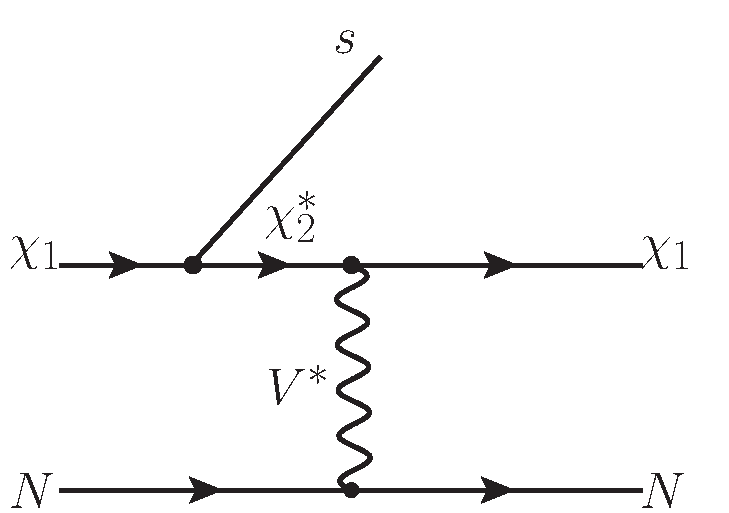
\includegraphics[width=\linewidth]{figures/LZ_3body_DM_signal_2}
    \end{minipage}
    \caption{Tree-level diagrams for $\chi_1 N\to\chi_1 N s$ with vector-mediator exchange, including scalar emission from the dark-fermion line before and after the exchange.}
    \label{fig:2_to_3_feynman}
\end{figure*}

\section{Direct detection}


\begin{figure}
	\centering
	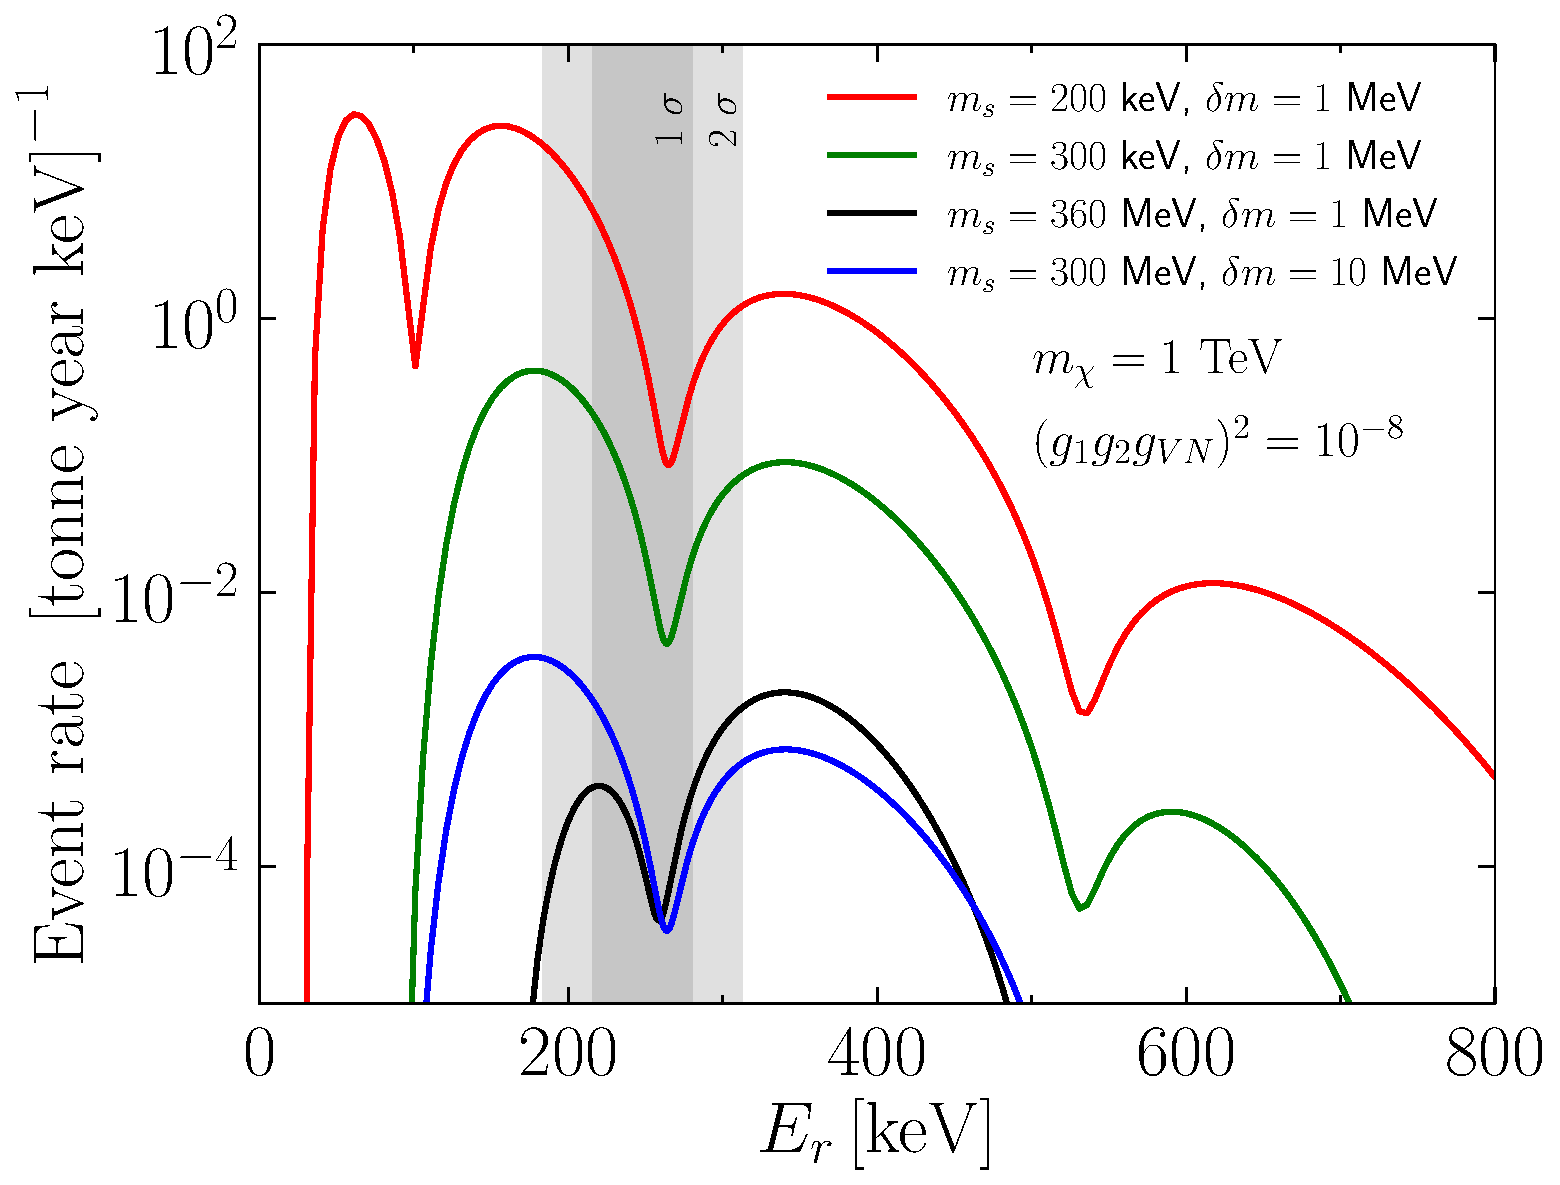
\includegraphics[width=0.8\linewidth]{figures/DM_signal}
	\caption{Event-rate spectra as functions of the nuclear recoil energy $E_R$ for the benchmark choices of $m_s$ and $\Delta m$ indicated in the legend, with $m_{\chi_1}=1\,\mathrm{TeV}$ and $(g_1g_2g_{VN})^2=10^{-8}$.}
	\label{fig:signal_spectrum}
\end{figure}

\begin{figure*}[t]
    \centering
    \begin{minipage}[t]{0.48\textwidth}
        \centering
        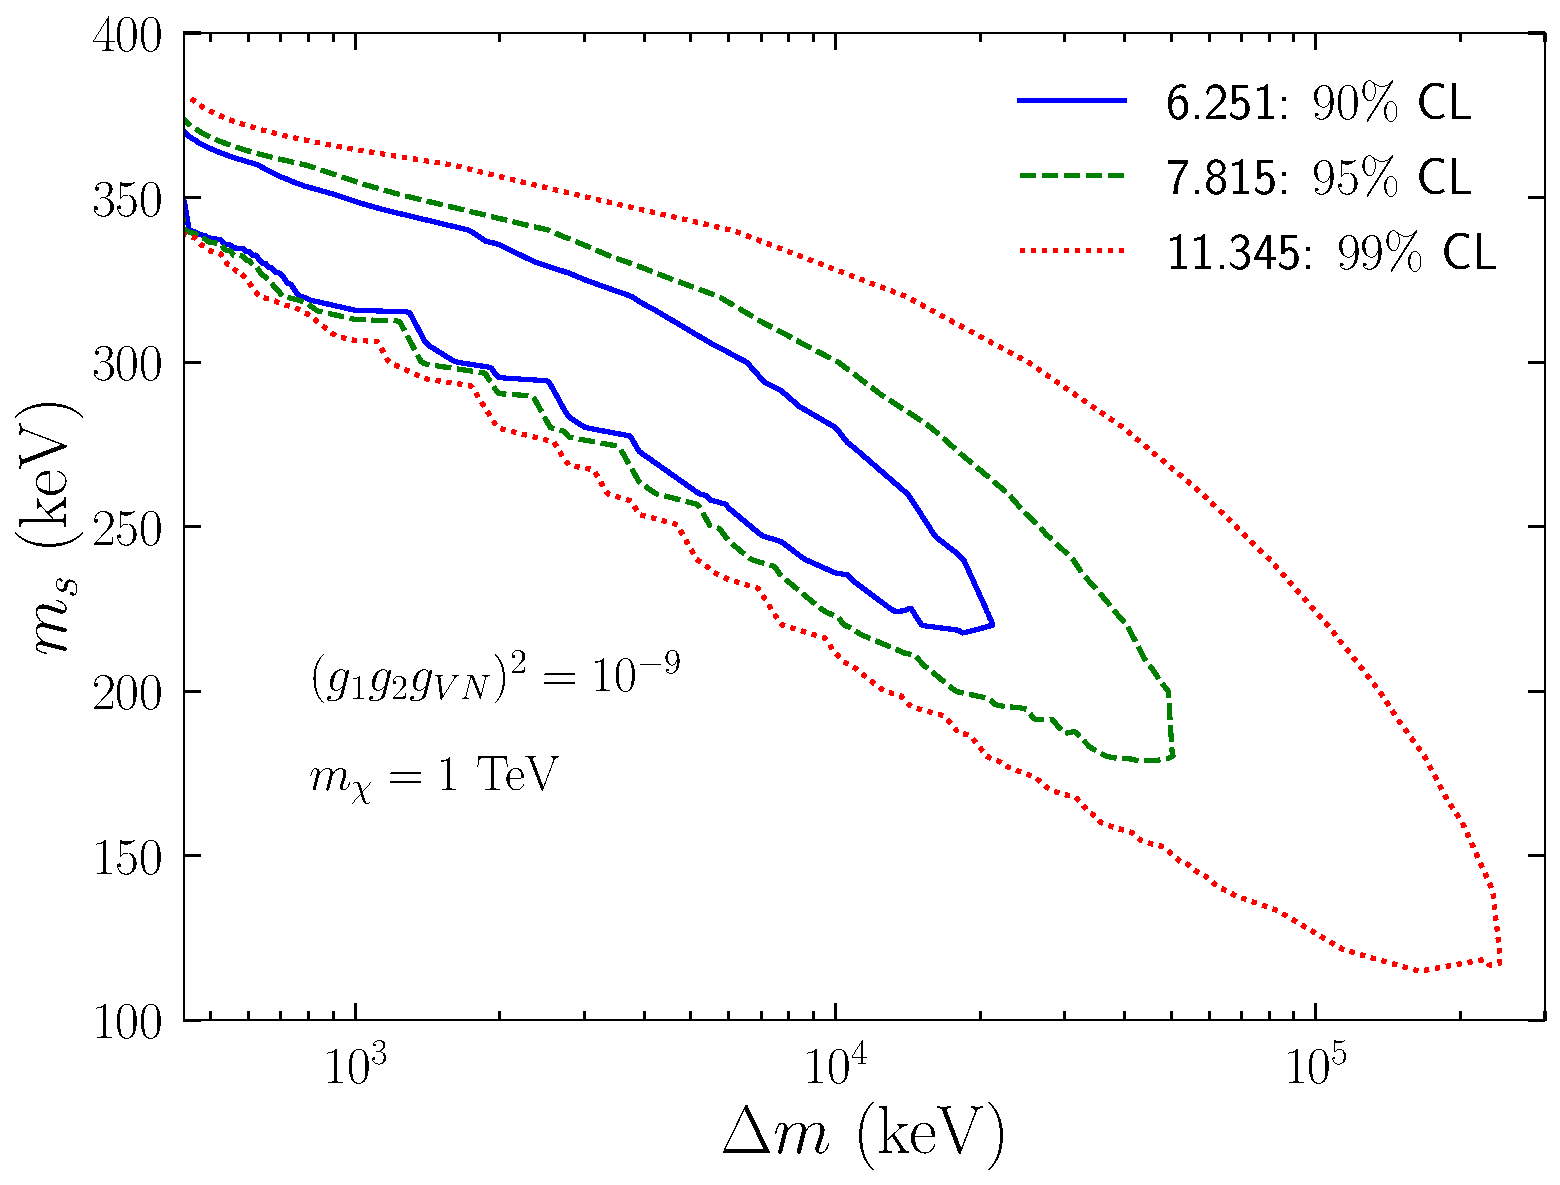
\includegraphics[width=\linewidth]{figures/3_body_contour_ms_deltam_1}
    \end{minipage}\hfill
    \begin{minipage}[t]{0.48\textwidth}
        \centering
        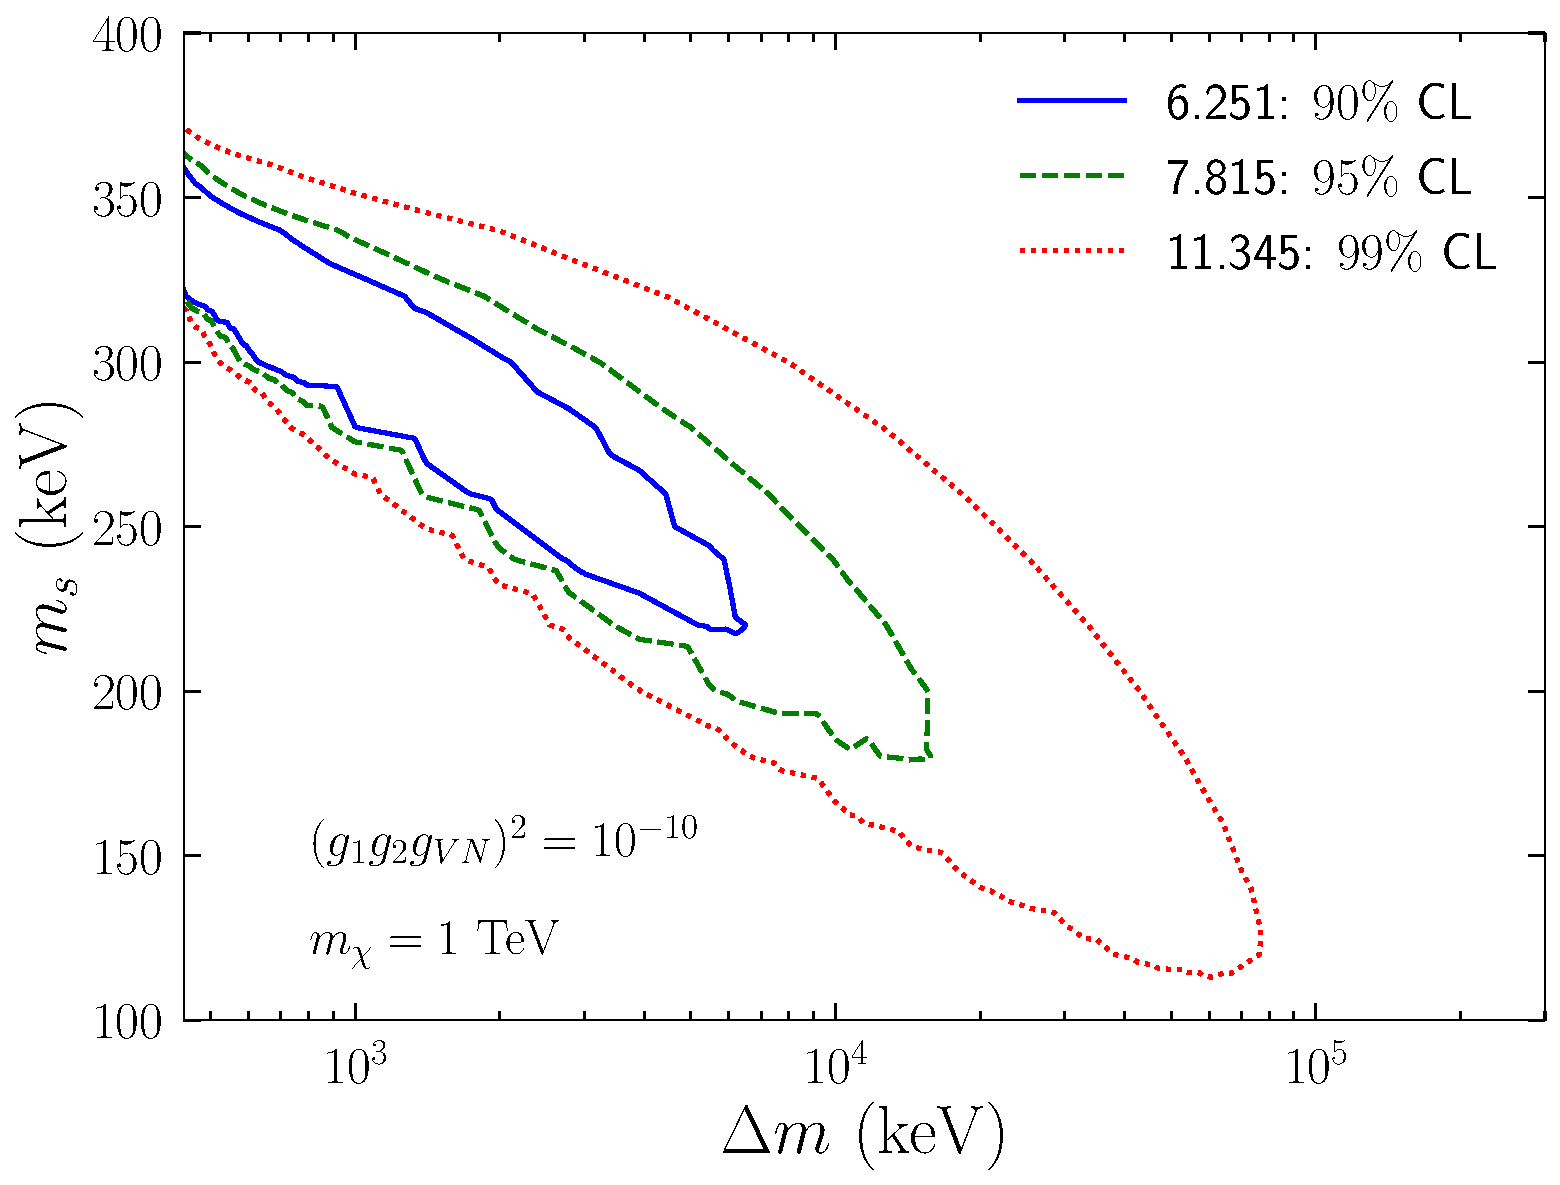
\includegraphics[width=\linewidth]{figures/3_body_contour_ms_deltam_2}
    \end{minipage}
    \caption{Confidence-level contours in the $(m_s,\Delta m)$ plane for $m_{\chi_1}=1\,\mathrm{TeV}$, with $(g_1g_2g_{VN})^2=10^{-9}$ (left panel) and $10^{-10}$ (right panel). The contour levels and confidence levels are indicated in the legend.}
    \label{fig:ms_delta_m_contour}
\end{figure*}

\begin{figure*}[t]
    \centering
    \begin{minipage}[t]{0.48\textwidth}
        \centering
        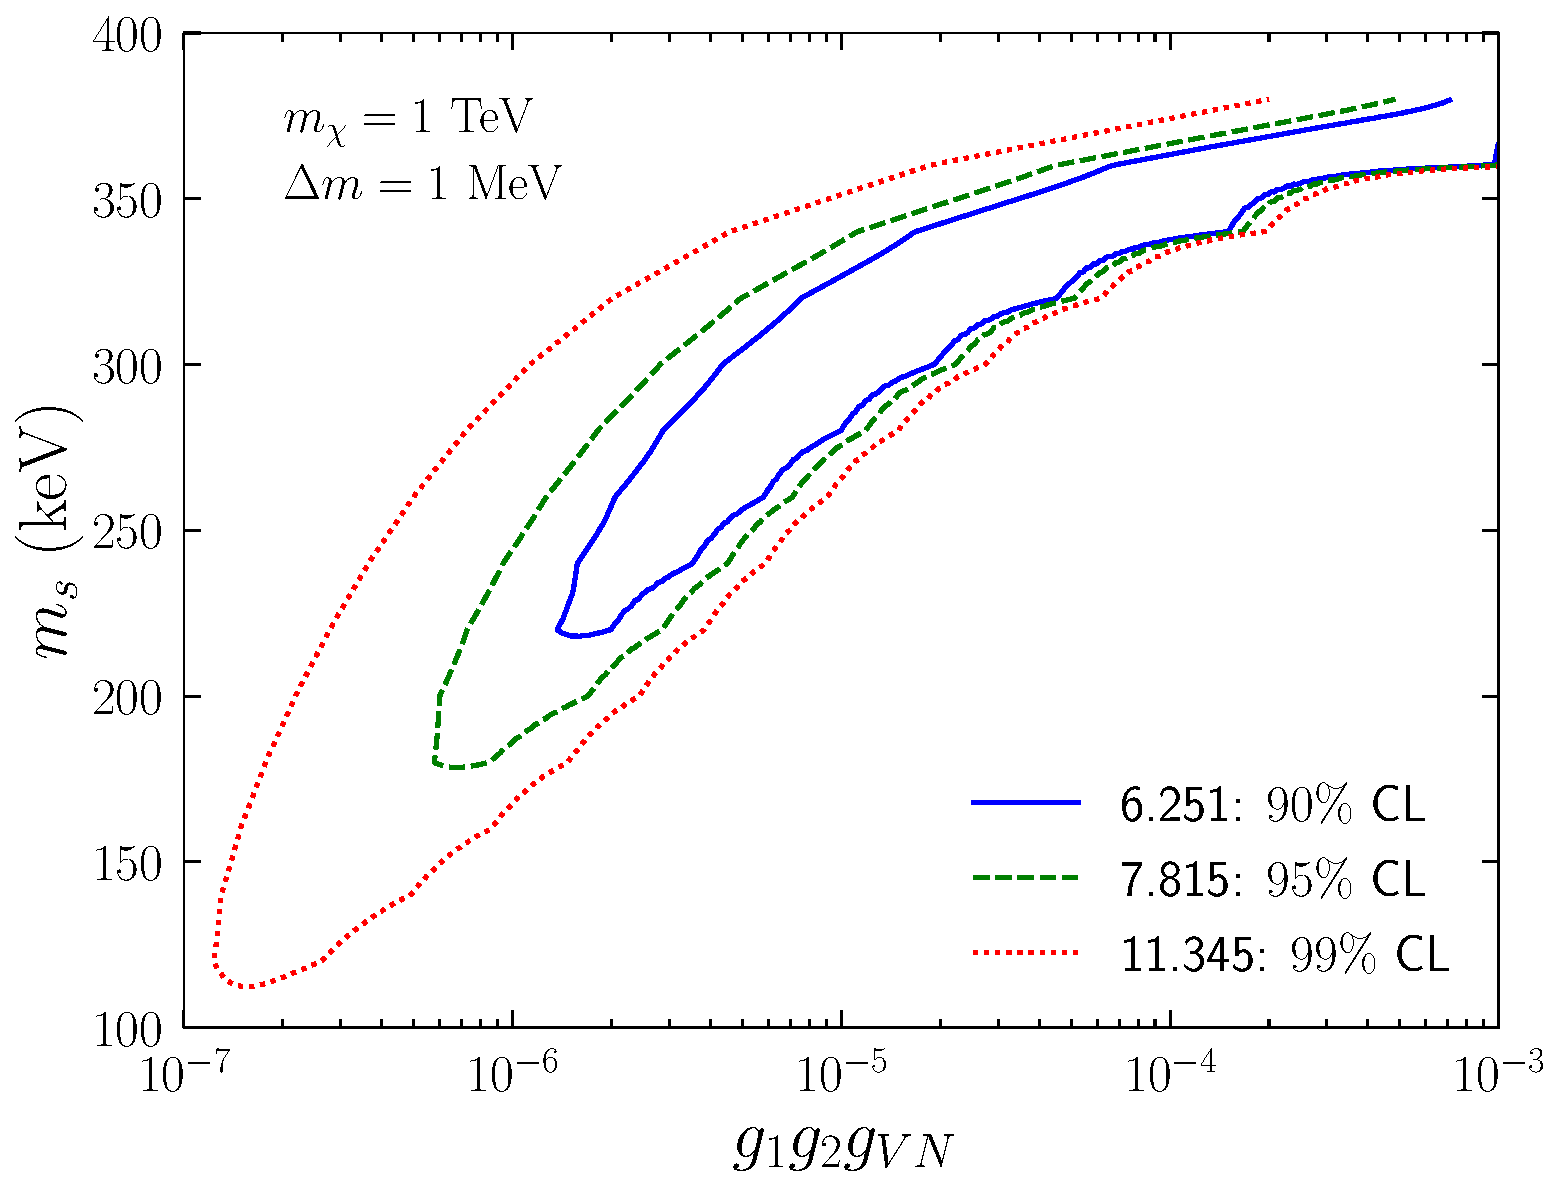
\includegraphics[width=\linewidth]{figures/3_body_contour_ms_coupling_1}
    \end{minipage}\hfill
    \begin{minipage}[t]{0.48\textwidth}
        \centering
        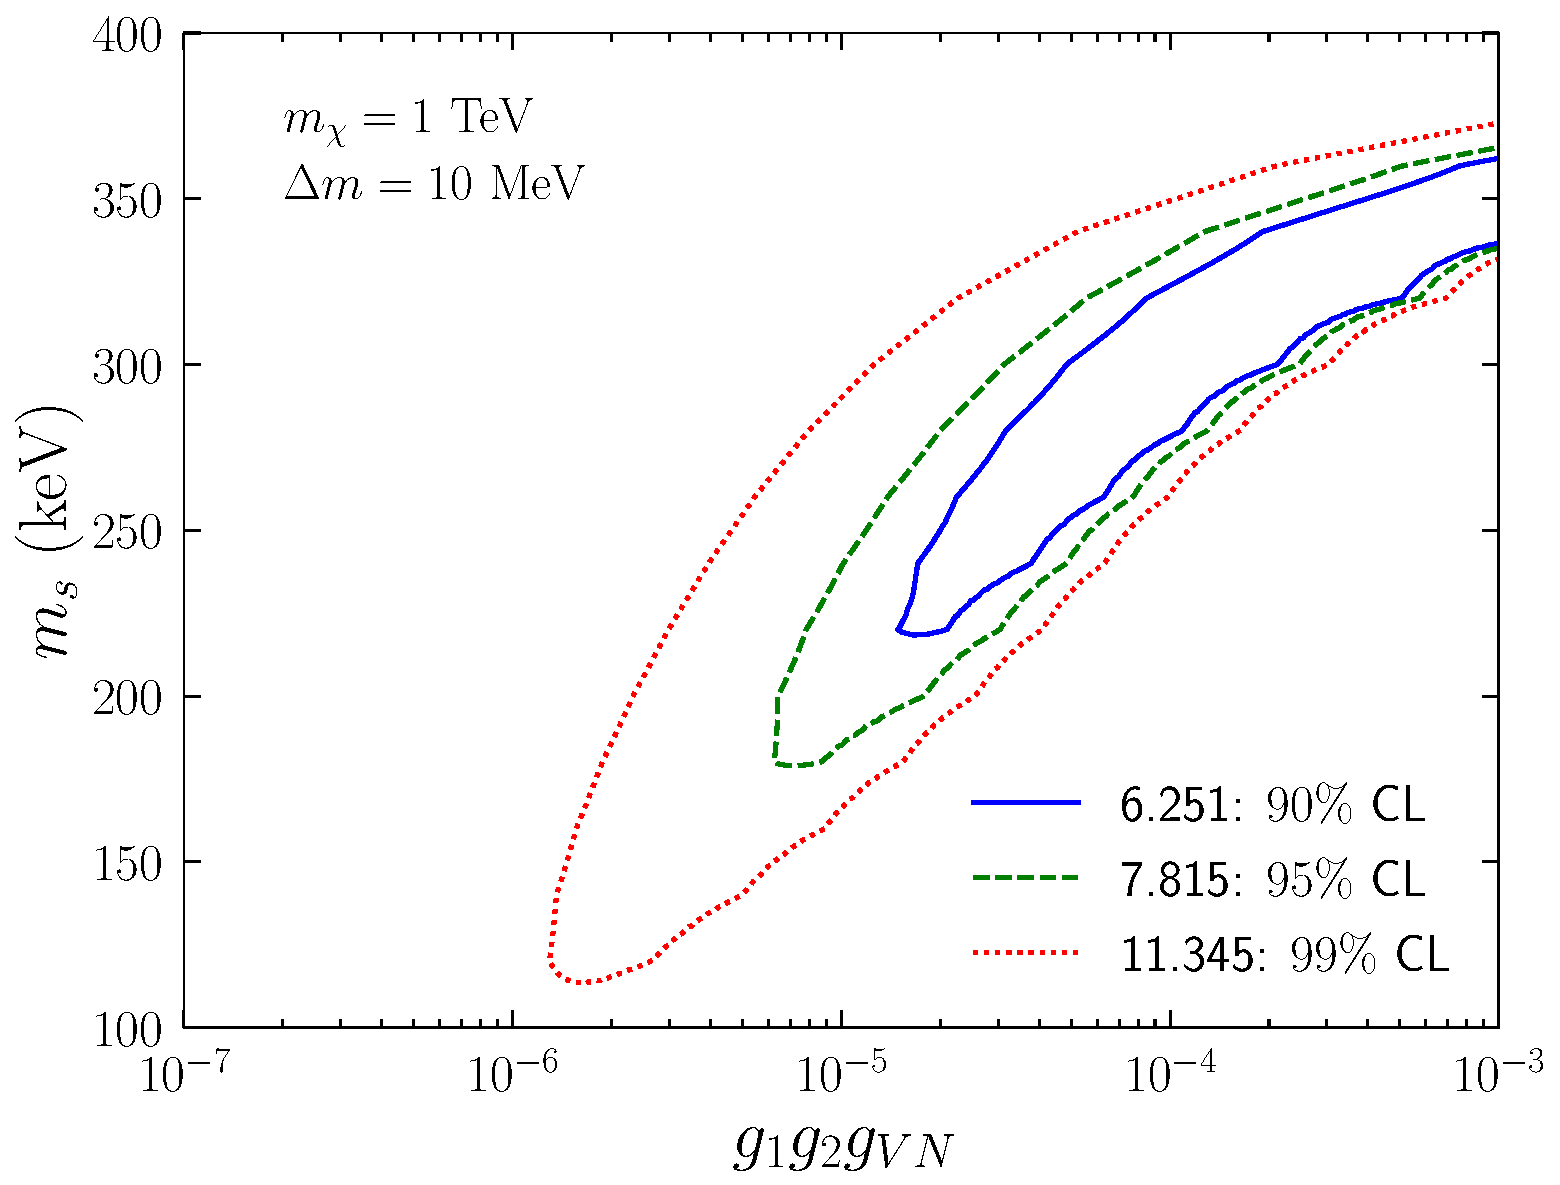
\includegraphics[width=\linewidth]{figures/3_body_contour_ms_coupling_2}
    \end{minipage}
    \caption{Confidence-level contours in the $(m_s,g_1g_2g_{VN})$ plane for $m_{\chi_1}=1\,\mathrm{TeV}$, with $\Delta m=1\,\mathrm{MeV}$ (left panel) and $10\,\mathrm{MeV}$ (right panel). The contour levels and confidence levels are indicated in the legend.}
    \label{fig:ms_coupling_m_contour}
\end{figure*}




\subsection{\texorpdfstring{$2 \to 3$}{2 to 3} cross section}
We consider
$\chi_1(p)+A(P)\to\chi_1(p')+A(P')+s(k)$,
with $q=P'-P$, $t=q^2=-2m_AE_R$, and $W^2=(p'+k)^2$.
Emission before and after vector exchange gives the fermion current
$\bar u(p')\Gamma^\mu u(p)$, where
\begin{equation}
\Gamma^\mu=
\frac{\gamma^\mu(\not p-\not k+m_{\chi_2})}{(p-k)^2-m_{\chi_2}^2}
+\frac{(\not p'+\not k+m_{\chi_2})\gamma^\mu}{W^2-m_{\chi_2}^2+i m_{\chi_2}\Gamma_{\chi_2}}.
\end{equation}
Here $\Gamma_{\chi_2}=\Gamma(\chi_2\to\chi_1 s)$ is evaluated at the pole mass.
Both diagrams and their interference are retained.

At leading order in the non-relativistic nuclear current, vector
exchange probes the coherent charge response.
For equal proton and neutron couplings, $g_p=g_n=g_{VN}$, we use the response function
$\mathcal R_A(E_R)=4\pi W_M^{00}(y)/(2J_A+1)$,
where $y=b_A^2m_AE_R/2$ and $\mathcal R_A(0)=A^2$
\cite{Anand:2013yka}.
The differential cross section is
\begin{equation}
\begin{split}
\frac{d\sigma_A}{dE_R}
={}&
\frac{m_A(g_1 g_2 g_{VN})^2}{256\pi^3p_{\chi_1}^2}
\\
&\quad\times
\frac{\mathcal R_A(E_R)}{(m_V^2+2m_AE_R)^2}
\\
&\times
\int_{W_{\min}^2}^{W_{\max}^2}dW^2\,
\sqrt{\lambda(W^2,m_{\chi_1}^2,m_s^2)}
\int_{-1}^{1}dz\,
\langle\mathcal L_{00}\rangle_{\varphi_*}.
\end{split}
\label{eq:radiative-recoil}
\end{equation}
Here $\mathcal L_{00}=\frac12\sum_{\rm spins}
|\bar u(p')\Gamma^0u(p)|^2$, with the time component defined in
the target rest frame.
The angles $z=\cos\theta_*$ and $\varphi_*$
specify the emitted scalar in the $\chi_1s$ rest frame,
with the polar axis along the incoming $\chi_1$ momentum;
$\langle\cdots\rangle_{\varphi_*}$ denotes the azimuthal average.
We use the dimensionless function
$\lambda(w,m_1^2,m_2^2)=
[1-(m_1+m_2)^2/w][1-(m_1-m_2)^2/w]$.
The integration limits are
\begin{align}
W_{\min}^2&=(m_{\chi_1}+m_s)^2,\\
W_{\max}^2&=m_{\chi_1}^2
+2p_{\chi_1}\sqrt{2m_AE_R+E_R^2}
-2(E_{\chi_1}+m_A)E_R,
\end{align}
where $E_{\chi_1}=m_{\chi_1}/\sqrt{1-v^2}$ and
$p_{\chi_1}=E_{\chi_1}v$.
We restrict the parameter space to $W_{\max}<m_{\chi_2}$
throughout the accessible halo phase space, excluding on-shell
$\chi_2$ production.

\appendix

\section{Post-freeze-out evolution}

We follow the light-sector evolution from the heavy-particle
freeze-out temperature $T_f$ through scalar decay. Sterile
neutrinos are denoted by $N_s$, distinct from nucleons.
We assume that $V$ remains in kinetic and chemical equilibrium
with the SM, $T_V=T_\gamma\equiv T$, and use Maxwell--Boltzmann
(MB) distributions
\[
f_V=e^{-E_V/T},
\quad
f_s=z_s e^{-E_s/T_s},
\quad
z_s=\frac{n_s}{n_s^{\rm eq}(T_s)}.
\]
The equilibrium density and mean energy are
\cite{EscuderoAbenza:2020cmq,Cirelli:2024ssz}
\begin{align}
n_i^{\rm eq}(T_i)
&=\frac{g_i m_i^2T_i}{2\pi^2}K_2(\frac{m_i}{T_i}),
\quad g_V=3,\quad g_s=1,
\\
u_i(T_i)
&=3T_i+m_i\frac{K_1(\frac{m_i}{T_i})}{K_2(\frac{m_i}{T_i})}.
\end{align}
Thus $\rho_s=n_su_s(T_s)$ and $P_s=n_sT_s$, including
out-of-equilibrium abundances within this closure.
We initialize $T_s=T_f$ and $n_s=n_s^{\rm eq}(T_f)$.

The heavy-particle $\chi_{1,2}, \bar\chi_{1,2}$ history is imported from
micrOMEGAs~\cite{Alguero:2023zol}:
\begin{align}
n_{\rm heavy}
=&\sum_{i=1,2}(n_{\chi_i}+n_{\bar\chi_i})
=s_{\rm SM}Y_{\rm heavy},\\
\rho_{\rm heavy}\simeq & \,\,m_{\chi_1}n_{\rm heavy}.
\end{align}
Here we neglect its kinetic energy, the small mass-splitting
correction, and feedback on the imported freeze-out history.
After freeze-out is complete, $n_{\rm heavy}\propto a^{-3}$.

While the SM species share a common temperature, the bath
thermodynamic functions and expansion rate are
\begin{align}
\rho_{\rm bath}
&=\rho_{\rm SM}+n_V^{\rm eq}u_V,
\\
P_{\rm bath}
&=Ts_{\rm SM}-\rho_{\rm SM}+n_V^{\rm eq}T,
\\
H^2
&=\frac{8\pi}{3M_{\rm Pl}^2}
\left(\rho_{\rm bath}+\rho_s+\rho_{N_s}+\rho_{\rm heavy}\right).
\end{align}
Here $M_{\rm Pl}$ is the unreduced Planck mass, and the SM
thermodynamic functions exclude dark-sector contributions.
SM chemical potentials are neglected.

For the post-freeze-out scalar evolution, we retain
$VV\leftrightarrow ss$ and $Vs\leftrightarrow Vs$, together
with scalar decay and inverse decay into sterile neutrinos.
The sources unrelated to sterile decay are therefore
\begin{align}
C_0 &= C_{\rm pair},\\
Q_0 &= Q_{\rm pair}+Q_{\rm elastic}.
\end{align}
Here $Q_0$ is the net energy transferred from the thermal
bath to the scalar population.

We neglect heavy-catalyzed conversion $Vh\leftrightarrow sh$ and the net scalar source from $\chi_2$ decays and
inverse decays, including the effect of excited-state regeneration through heavy-particle collisions and scattering with the SM bath.
While the final numerical result $\Delta N_{\rm eff}$ for the benchmark considered here does not show much difference, we therefore neglect it in the calculation.

Including the decay terms defined below,
$C_s=C_0+C_{\rm dec}$ and $Q_s=Q_0+Q_{\rm dec}$,
the scalar moment equations are~\cite{EscuderoAbenza:2020cmq}
\begin{align}
\dot n_s+3Hn_s&=C_s,
\\
\dot\rho_s+3H(\rho_s+P_s)&=Q_s.
\end{align}
With $c_{V,s}={\rm d}u_s/{\rm d}T_s$, the temperature equations
are
\begin{align}
\dot T_s
&=\frac{Q_s-u_sC_s-3Hn_sT_s}{n_sc_{V,s}},
\\
\dot T
&=-\frac{3H(\rho_{\rm bath}+P_{\rm bath})+Q_0}
{{\rm d}\rho_{\rm bath}/{\rm d}T}.
\end{align}
Positive sources add scalar number or energy. The bath
loses only $Q_0$, not the internal exchange $Q_{\rm dec}$.
Residual heavy-annihilation heating is neglected.

%All cross sections below are averaged over initial polarizations and summed over final polarizations, including the appropriate identical-final-state factors. 
For $VV\leftrightarrow ss$, we define the equilibrium event
density~\cite{Cirelli:2024ssz}
\begin{align}
\gamma_{VV\to ss}^{\rm eq}(T)
=&\frac12[n_V^{\rm eq}(T)]^2
\langle\sigma v_{\rm Mol}\rangle
\nonumber\\
=&\frac{9T}{64\pi^4}
\int_{s_{\min}}^\infty {\rm d}s\,
s^{3/2}\lambda(s,m_V^2,m_V^2)\nonumber\\
& \times\sigma_{VV\to ss}(s)K_1(\frac{\sqrt{s}}{T}),
\end{align}
where $s_{\min}=\max(4m_V^2,4m_s^2)=4m_V^2$ for our benchmark. 
%The initial-pair factor $1/2$ avoids double counting; the final-state factor is already contained in $\sigma_{VV\to ss}$.
The corresponding total-energy moment is
\cite{Fernandez:2021iti}
\begin{align*}
\mathcal E_{VV\to ss}^{\rm eq}(T)
=&\frac{9T}{64\pi^4}
\int_{s_{\min}}^\infty {\rm d}s\,
s^2\lambda(s,m_V^2,m_V^2)\\
& \times\sigma_{VV\to ss}(s)K_2(\frac{\sqrt{s}}{T}).
\end{align*}
Detailed balance then gives
\begin{align}
C_{\rm pair}
&=2\left[\gamma_{VV\to ss}^{\rm eq}(T)
-z_s^2\gamma_{VV\to ss}^{\rm eq}(T_s)\right],
\\
Q_{\rm pair}
&=\mathcal E_{VV\to ss}^{\rm eq}(T)
-z_s^2\mathcal E_{VV\to ss}^{\rm eq}(T_s).
\end{align}
No additional factor of two enters $Q_{\rm pair}$, since
$\mathcal E^{\rm eq}$ weights the total energy per reaction.
For temperature-independent microscopic inputs, the moments
needed for the relaxation analysis follow from
\[
\mathcal E^{\rm eq}
=T^2\frac{{\rm d}\gamma^{\rm eq}}{{\rm d}T},
\quad
\mathcal E_2^{\rm eq}
=T^2\frac{{\rm d}\mathcal E^{\rm eq}}{{\rm d}T}.
\]

For $V(p_1)s(p_2)\to V(p_3)s(p_4)$, starred quantities
refer to the center-of-mass frame, while unstarred energies
refer to the cosmological frame. The scalar energy and
momentum in the former are
\[
E_2^*=E_4^*=\frac{s+m_s^2-m_V^2}{2\sqrt{s}},
\quad
p_*=\frac{\sqrt{s\lambda(s,m_V^2,m_s^2)}}{2}.
\]
With boost factor $\gamma_B=(E_1+E_2)/\sqrt{s}$, averaging
over the scattering azimuth gives
\[
\overline{E_4-E_2}
=(\gamma_BE_2^*-E_2)(1-\cos\theta_*).
\]
This motivates the momentum-transfer cross section
\[
\sigma_T(s)
=\int {\rm d}\Omega_*\,(1-\cos\theta_*)
\frac{{\rm d}\sigma_{Vs\to Vs}}{{\rm d}\Omega_*}.
\]
After integration over the incoming orientations,
\[
\begin{aligned}
Q_{\rm elastic}
={}&\frac{3z_s}{32\pi^4}
\int_{(m_V+m_s)^2}^\infty {\rm d}s\,s\\
&\quad\times\sqrt{\lambda(s,m_V^2,m_s^2)}
\sigma_T(s)\mathcal I_E(s).
\end{aligned}
\]
where
\begin{align*}
\mathcal I_E(s)
= &\int_{\mathcal D(s)}{\rm d}E_1\,{\rm d}E_2\,
e^{-E_1/T-E_2/T_s}\\
&\times \left[(E_1+E_2)\frac{s+m_s^2-m_V^2}{2s}-E_2\right].
\end{align*}
Writing $E=E_1+E_2$ and $P=\sqrt{E^2-s}$, the integration
domain is
\[
E\ge\sqrt{s},\quad aE-bP\le E_2\le aE+bP,
\]
\[
a=\frac{s+m_s^2-m_V^2}{2s},\quad
b=\frac{\sqrt{\lambda(s,m_V^2,m_s^2)}}{2}.
\]
The remaining energy integrals are evaluated in the unequal-temperature
MB formalism of Ref.~\cite{BeauchesneKats2021}, giving
\[
\mathcal I_E(s)
=\frac{s^2\lambda^{3/2}(s,m_V^2,m_s^2)}{4}
\left(\frac1{T_s}-\frac1T\right)\frac{K_2(w)}{w^2},
\]
\[
w^2=\frac{m_V^2}{T^2}+\frac{m_s^2}{T_s^2}
+\frac{s-m_V^2-m_s^2}{TT_s}.
\]
Hence
\begin{align}
Q_{\rm elastic}
={}&\frac{3z_s}{128\pi^4}
\left(\frac1{T_s}-\frac1T\right)
\nonumber\\
&\times\int_{(m_V+m_s)^2}^\infty {\rm d}s\,
s^3\lambda^2(s,m_V^2,m_s^2)
\sigma_T(s)\frac{K_2(w)}{w^2}.
\end{align}
This term conserves scalar number and transfers energy
toward the colder population, vanishing at $T_s=T$.

\subsection{Scalar decay and dark radiation}

We introduce one effectively massless Majorana sterile
neutrino through
\[
\mathcal L_{\rm dec}
=-\frac{y_\nu}{2}s\overline{N_s}N_s,
\quad
\Gamma_s=\frac{y_\nu^2m_s}{16\pi},
\]
where $\Gamma_s$ is the rest-frame width. The sterile
population is described by an MB moment closure,
\[
f_{N_s}=z_{N_s}e^{-p/T_{N_s}},
\quad
n_{N_s}^{\rm eq}=\frac{2T_{N_s}^3}{\pi^2},
\]
\[
z_{N_s}=\frac{n_{N_s}}{n_{N_s}^{\rm eq}},
\quad
\rho_{N_s}=3n_{N_s}T_{N_s}.
\]
Here, chemical equilibrium is not imposed.

The decay and inverse-decay sources into $s$ are
\cite{EscuderoAbenza:2020cmq}
\begin{align}
C_{\rm dec}
&=\frac{\Gamma_s m_s^2}{2\pi^2}
\left[z_{N_s}^2T_{N_s}K_1(\frac{m_s}{T_{N_s}})
-z_sT_sK_1(\frac{m_s}{T_s})\right],
\label{eq:scalar-decay-number}
\\
Q_{\rm dec}
&=\frac{\Gamma_s m_s^3}{2\pi^2}
\left[z_{N_s}^2T_{N_s}K_2(\frac{m_s}{T_{N_s}})
-z_sT_sK_2(\frac{m_s}{T_s})\right].
\label{eq:scalar-decay-energy}
\end{align}
The inverse terms vanish for an empty sterile population.
Without inverse decays, $Q_{\rm dec}=-m_s\Gamma_s n_s$,
since the energy weight cancels the decay time-dilation
factor. Together with the scalar equations above, we evolve
\begin{align}
\dot n_{N_s}+3Hn_{N_s}&=-2C_{\rm dec},
\\
\dot\rho_{N_s}+4H\rho_{N_s}&=-Q_{\rm dec}.
\label{eq:sterile-energy-evolution}
\end{align}
We initialize $n_{N_s}=\rho_{N_s}=0$ at $T_f$ and carry
both moments continuously through the decay epoch.
For $n_{N_s}>0$, $T_{N_s}=\rho_{N_s}/(3n_{N_s})$.
The coupled equations satisfy
\begin{align}
\frac{{\rm d}}{{\rm d}t}\left[a^3(2n_s+n_{N_s})\right]
&=2a^3C_0,
\\
\frac{{\rm d}}{{\rm d}\ln a}
\left[a^4(\rho_s+\rho_{N_s})\right]
&=a^4\left(\rho_s-3P_s+\frac{Q_0}{H}\right).
\end{align}
Thus internal decays conserve energy, while a
nonrelativistic scalar can increase the comoving dark
radiation energy before disappearing.

During the MeV epoch, $V$ is exponentially suppressed.
The electromagnetic bath contains photons and electrons/
positrons, with Fermi--Dirac statistics for the latter.
We approximate active-neutrino decoupling as instantaneous
at $T_{\nu,\rm dec}=2\,{\rm MeV}$, with
$\rho_{\nu_a}=7\pi^2T_\nu^4/40$ for three species.
Before decoupling, $T_\nu=T_\gamma$ and
\[
\dot T_\gamma
=-\frac{3H(\rho_{\rm EM}+P_{\rm EM}+4\rho_{\nu_a}/3)+Q_0}
{{\rm d}\rho_{\rm EM}/{\rm d}T_\gamma+4\rho_{\nu_a}/T_\gamma}.
\]
After decoupling,
\[
\dot T_\nu=-HT_\nu,
\quad
\dot T_\gamma
=-\frac{3H(\rho_{\rm EM}+P_{\rm EM})+Q_0}
{{\rm d}\rho_{\rm EM}/{\rm d}T_\gamma}.
\]
The expansion rate in this epoch is
\[
H^2=\frac{8\pi}{3M_{\rm Pl}^2}
\left(\rho_{\rm EM}+\rho_{\nu_a}+\rho_s
+\rho_{N_s}+\rho_{\rm heavy}\right).
\]

After scalar decay and electron--positron annihilation
are complete, we evaluate
\begin{equation}
\Delta N_{\rm eff}
=\frac{\rho_{N_s}}
{\frac78(\frac4{11})^{4/3}\rho_\gamma},
\quad
\rho_\gamma=\frac{\pi^2}{15}T_\gamma^4.
\label{eq:sterile-delta-neff}
\end{equation}
We quote this additional contribution separately, or use
$N_{\rm eff}\simeq3.045+\Delta N_{\rm eff}$ with the SM
reference value of Ref.~\cite{EscuderoAbenza:2020cmq}.
This does not include a precision recalculation of active
neutrino reheating in the presence of dark radiation.

For the reference benchmark, switching off heavy-pair
regeneration or enhancing its rate by two orders of
magnitude changes $\Delta N_{\rm eff}$ by approximately
one percent. A separate quantum-equilibrium thermodynamic
check gives $\Delta N_{\rm eff}\simeq0.046$, compared with
$0.043$ in the MB treatment. These sensitivity checks
support the estimated radiation contribution of a few
$\times10^{-2}$, without implying percent-level precision.


\bibliography{ref}
\bibliographystyle{utphys28mod}
\end{document}
